\section{Introduction}

% \note{jk: you need two paragraphs in intro to describe the problem statement.
% 	What I read in the first paragraph is not relevant with the problem that your
% 	thesis solves. The problem is: 1. Data analytics and search engines running on JVM need large heaps.
% 	2. A promising solution for large heaps that do not increase the GC cost is dual-heap designes, such as TeraHeap. Explain how does TeraHeap work and explain the problem of DRAM division.
% 	3. Then put a paragraph describing in high level your solution and how does this solution work.
% 	4. write where you implement your solution and provide some high-level results.
% }

Widely-used data analytics and search engines such as \textbf{Apache Lucene}
\cite{klinaftakis2025thesis} and \textbf{Apache Spark} run over Java virtual
machines (JVM). They require large heaps in order to be able to process large
datasets. \note{jk: Such systems require to host large compute caches. For
	example, Lucene maintains a query cache to store frequently queries to avoid
	their recomputation. Similarly, Spark maintains on-heap cache to store
	intermediate results to avoid recomputation. However, large-heaps require large
	amount of DRAM but DRAM capacity scalining is limited. Also, large-heaps
	requires expensive GC scans and compactions}.

A solution for large heaps that does not add overheads to the GC cost is
dual-heap designs, such as TeraHeap \note{jk: add citation!!}. TeraHeap extends
G1, the default garbage collector of OpenJDK to use two heaps: a primary heap
(H1) in DRAM and a second high capacity heap (H2) memory-mapped over a fast
storage device which is acccessed though OS page cache. G1 scans and compacts
objects in H1, but avoid GC scans over H2. The DRAM division between the main
heap and the pagecache must happen at the beginning of an execution statically,
which presents a problem since the system can not adapt in phases with
different memory and I/O demands.

\note{say the goal of this paragraph!! then show the figure and explain the results}
Figure~\ref{fig:vanilla-dram-underutilization} illustrates a native Lucene
benchmark using a total of 8GB of DRAM, evenly split between H1 and the OS page
cache. At the beginning of the run, the heap usage rapidly spikes, indicating
that an increased number of GC cycles is occurring. As the benchmark execution
progresses, the heap usage stabilizes at a much lower level, suggesting that
part the heap could be shrunk and the page increased to hold more data from the
H2 file, without massively affecting GC performance. This behavior highlights
the limitations of static partitioning.
\begin{figure}[htbp]
	\centering
	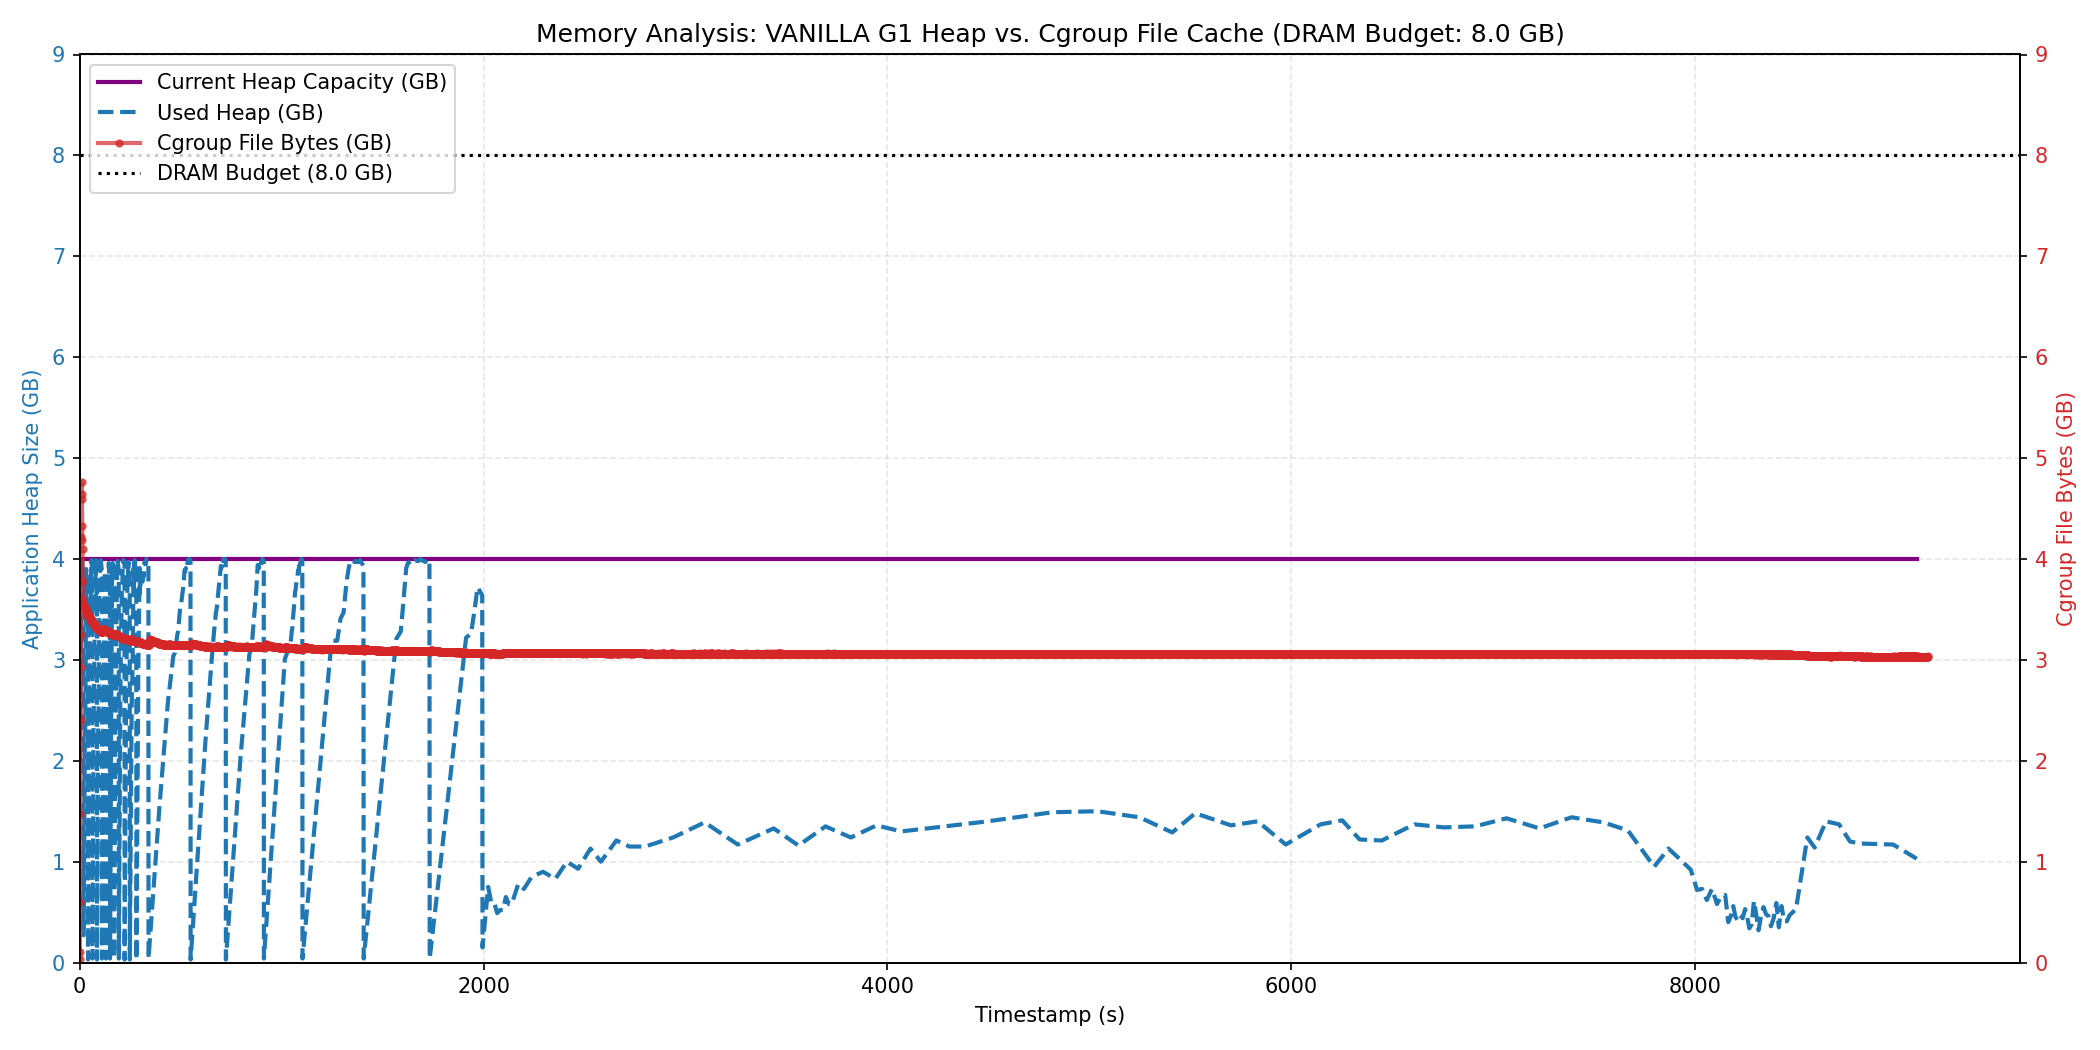
\includegraphics[width=1\linewidth]{fig/combined_memory_timeline_vanilla_g1.png}
	\caption{
		M1 Lucene benchmark with static DRAM configuration of 4GB H1 and 4GB pagecache.
	}
	\label{fig:vanilla-dram-underutilization}
\end{figure}

To address this limitation, we port \textbf{FlexHeap} to our system, a dynamic
resizing policy that operates at runtime by dividing execution into sampling
intervals. During each interval, it tracks the number of CPU time consumed by GC
\note{jk: first say garbage collection and then defind the accronym. then in the rest of the text use the acronym.}
(garbage collection) and the I/O overheads including I/O caused by accesses to
the (H2) memory-mapped file. At the end of each interval, it compares the
percent change between the two metrics, relative to the previous intervals. If
garbage collection overhead has increased more than I/O stalls, FlexHeap
signals G1 to grow the H1 heap to relieve GC pressure. Inversely, if I/O delays
have increased, a shrink heap action is invoked, shifting the remaining memory
towards the pagecache, via cgroups, to reduce evictions and hold more data from
the H2 file.

\note{jk: write in which version of OpenJDK you have impement FlexHeap. Then
	discuss the high-level results}Across Lucene's and Spark's benchmarks, FlexHeap
reports execution time improvements up to 70\% and 9\% accordingly.

\note{jk: Here write in bullet points the contributions. For example, we show
	the problem of dynamic dram partitioning in tiered managed heaps. A second
	contibution is the implementation of FlexHeap on top of TeraHeap}
